\documentclass{report}
%\usepackage{llncsdoc}
\usepackage{graphicx}

\usepackage{caption}
\usepackage{subcaption}
\captionsetup{compatibility=false}

\usepackage[bookmarks]{hyperref}

\usepackage[backend=bibtex,style=verbose-trad2]{biblatex}
\addbibresource{biblio.bib}
%

\begin{document}

\newpage

\title{Pick and Place}
\author{Group 8\\\small{email@student.sdu.dk}\\University of Southern Denmark}
\date{May 28, 2015}
\maketitle

\begin{abstract}
Text
\end{abstract}

\tableofcontents
\pagebreak

\chapter{Vision}
\section{Known object}
For this project we have two objects, which are created using the 3D design software called Autodesk Inventor 3D CAD. The result of this gave us an accurate 3D model which we were able to recreate using a 3D printer. The end result was an object the robot is able to pick up, with known dimensions.

\subsection{3D to 2D}
Since the world observed by a camera is 2D, some work has to be done to be able to perceive the 3D object. To do this, the objects were rendered from a multitude of different angles. The simple nature of these objects made it so only a few viewing angles were needed to capture the essence of the 3-dimensional shape.
The first object used is a sphere, this shape was chosen as this is the least complicated shape to test with. No matter from which angle the object is observed, the shape will always be the same. See Figure~\ref{fig:2dSphere}.
The second object, a cube, is a bit more complicated shape. When a cube is observed from a different angle, the shape will look different. For this object it was necessary to render images from different angles. A small selection of the resulting images can be seen in Figure~\ref{fig:2dCube1}, Figure~\ref{fig:2dCube2} and Figure~\ref{fig:2dCube3}.

\begin{figure}[h!]
\center
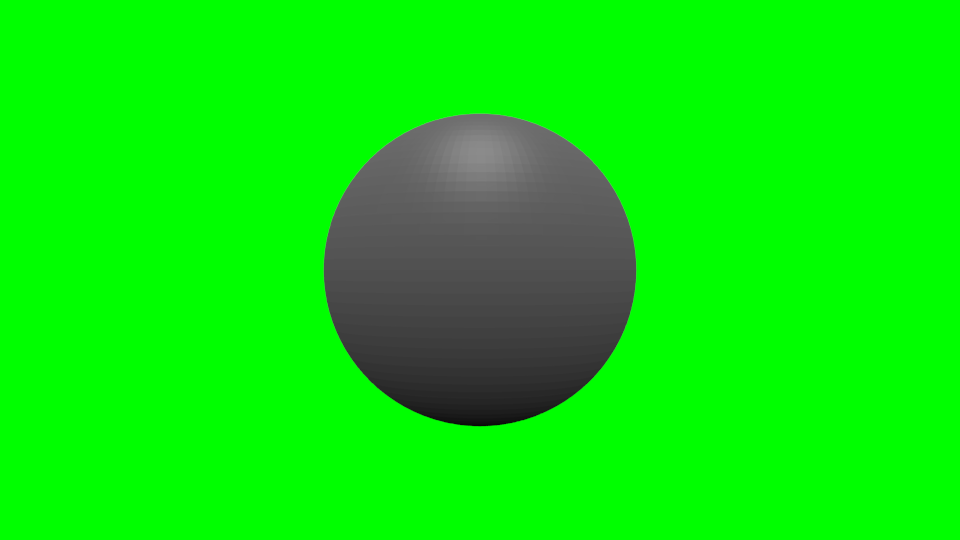
\includegraphics[width=.5\textwidth]{../images/0001.png}
\caption[]{2D image derived from 3D sphere}
\label{fig:2dSphere}
\end{figure}

\begin{figure}[h!]
\center
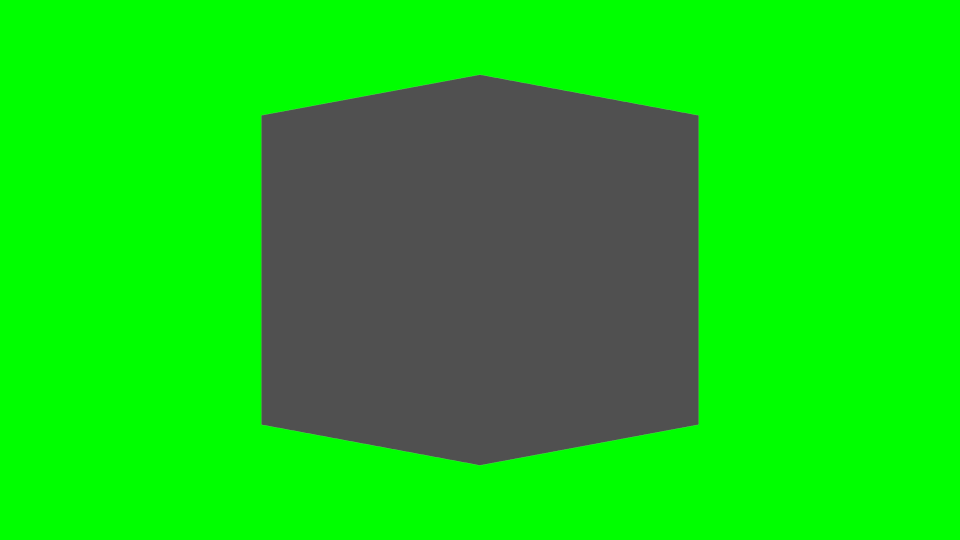
\includegraphics[width=.25\textwidth]{../images/cube_01/0001.png}
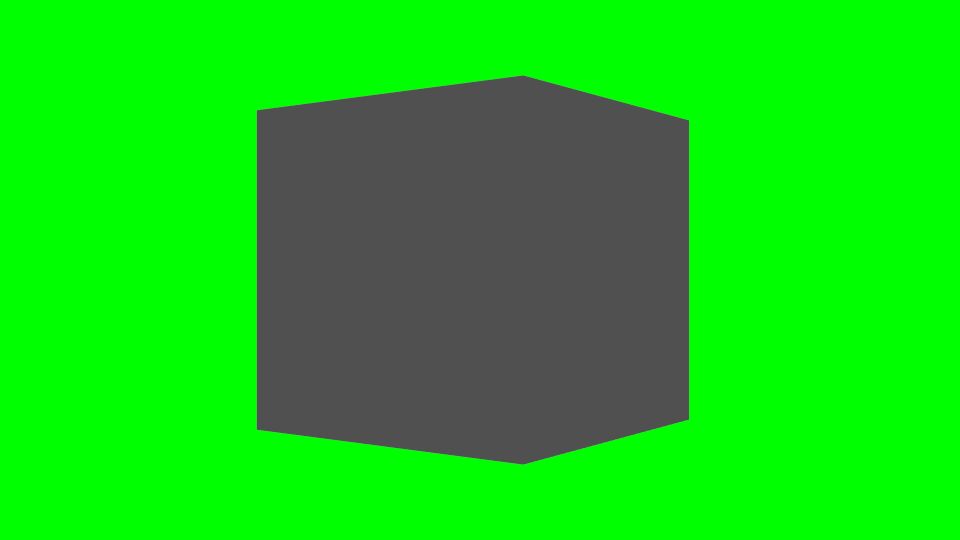
\includegraphics[width=.25\textwidth]{../images/cube_01/0010.png}
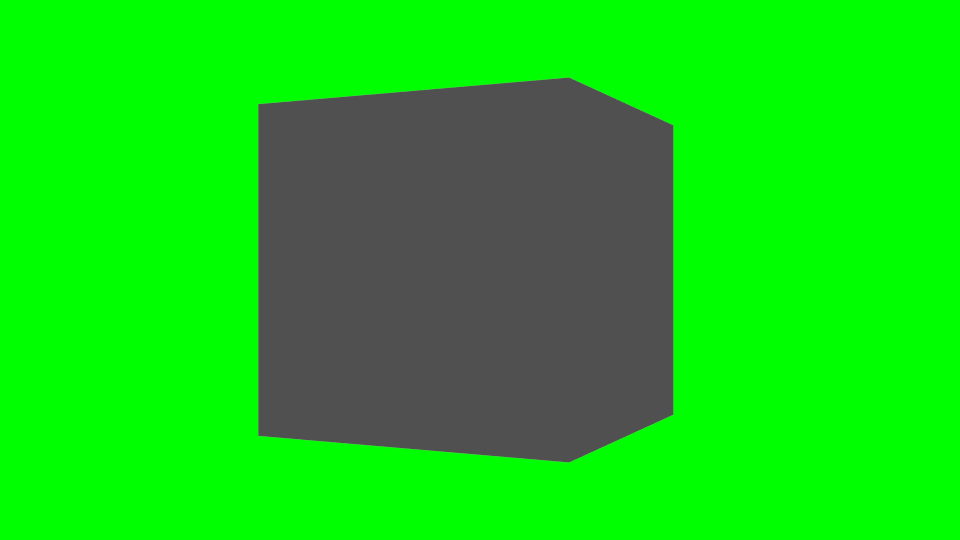
\includegraphics[width=.25\textwidth]{../images/cube_01/0020.png}
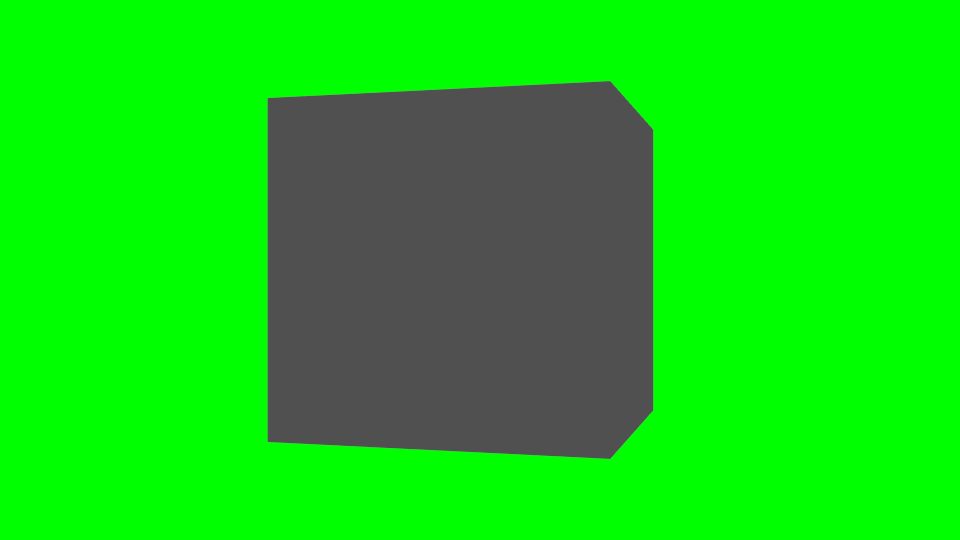
\includegraphics[width=.25\textwidth]{../images/cube_01/0030.png}

\includegraphics[width=.25\textwidth]{../images/cube_01/0040.png}
\caption[]{2D image derived from 3D cube}
\label{fig:2dCube1}
\end{figure}

\begin{figure}[h!]
\center
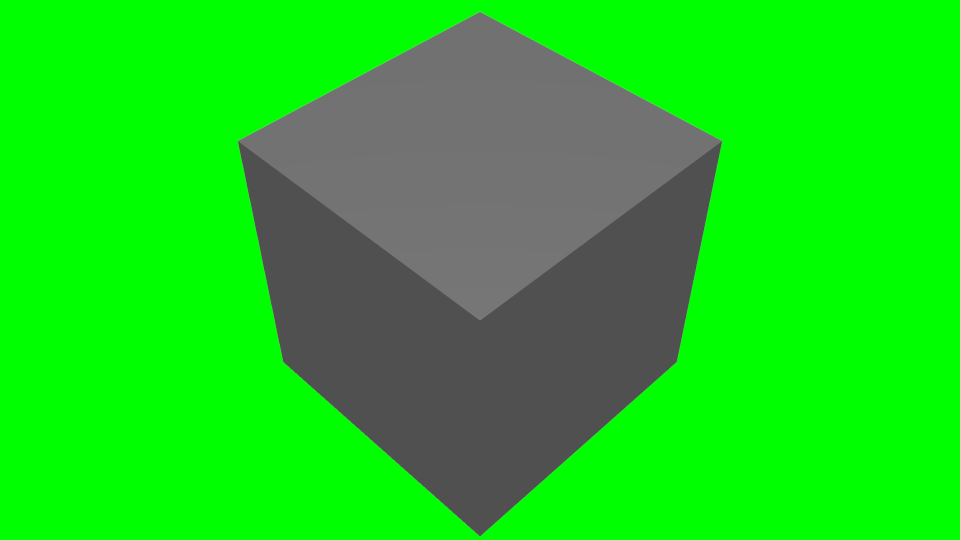
\includegraphics[width=.25\textwidth]{../images/cube_02/0001.png}
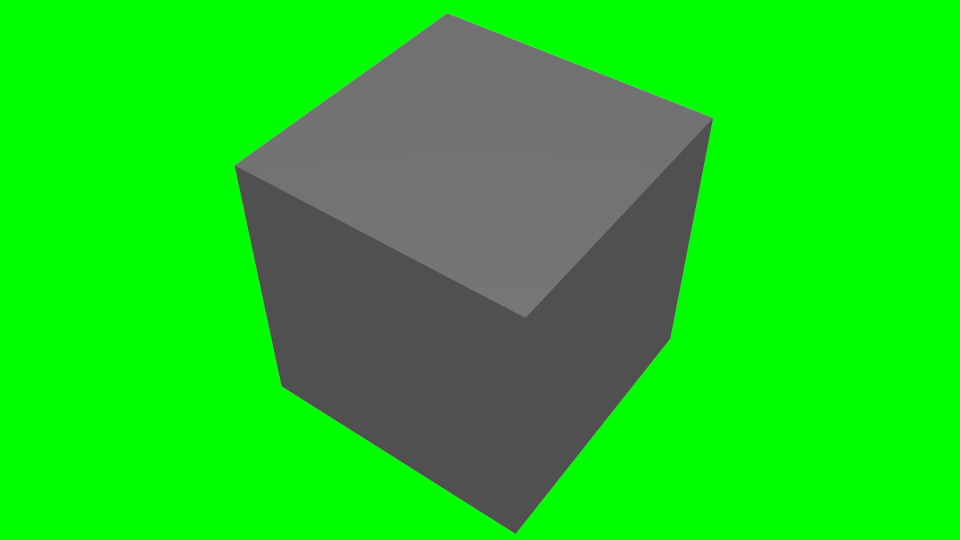
\includegraphics[width=.25\textwidth]{../images/cube_02/0010.png}
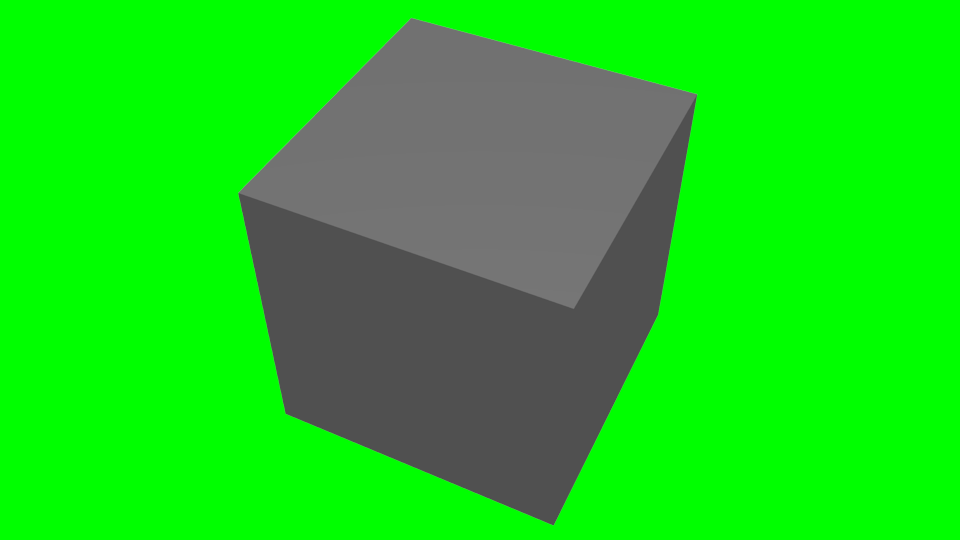
\includegraphics[width=.25\textwidth]{../images/cube_02/0020.png}
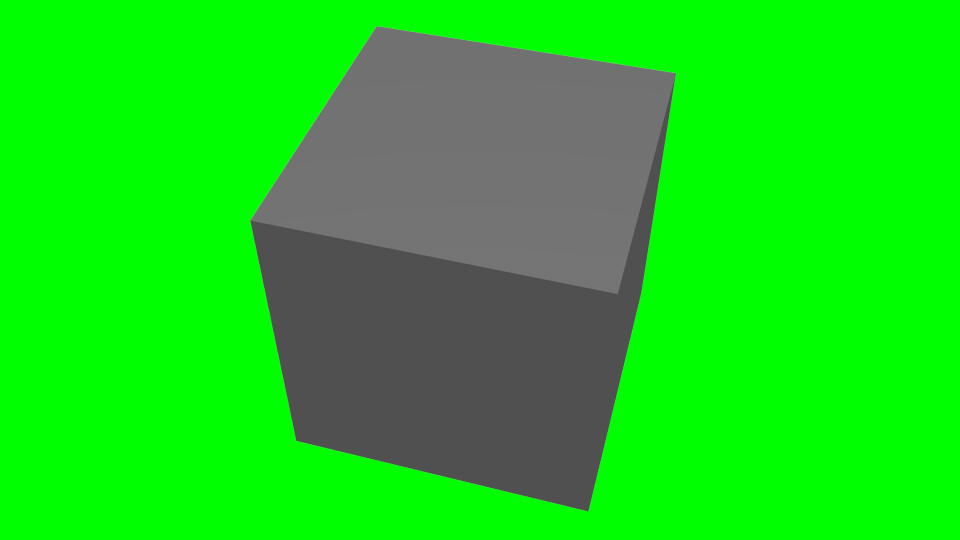
\includegraphics[width=.25\textwidth]{../images/cube_02/0030.png}

\includegraphics[width=.25\textwidth]{../images/cube_02/0040.png}
\caption[]{2D image derived from 3D cube}
\label{fig:2dCube2}
\end{figure}

\begin{figure}[h!]
\center
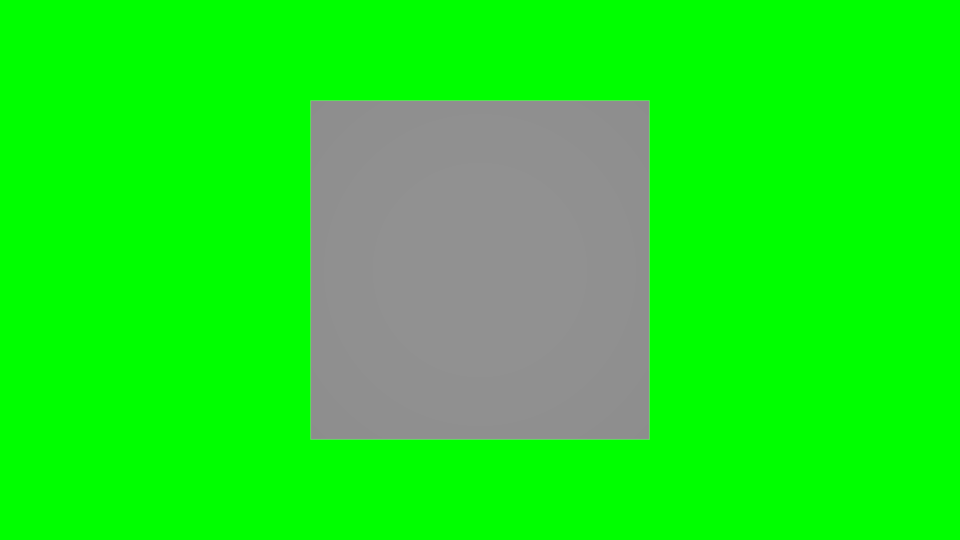
\includegraphics[width=.25\textwidth]{../images/cube_03/0001.png}
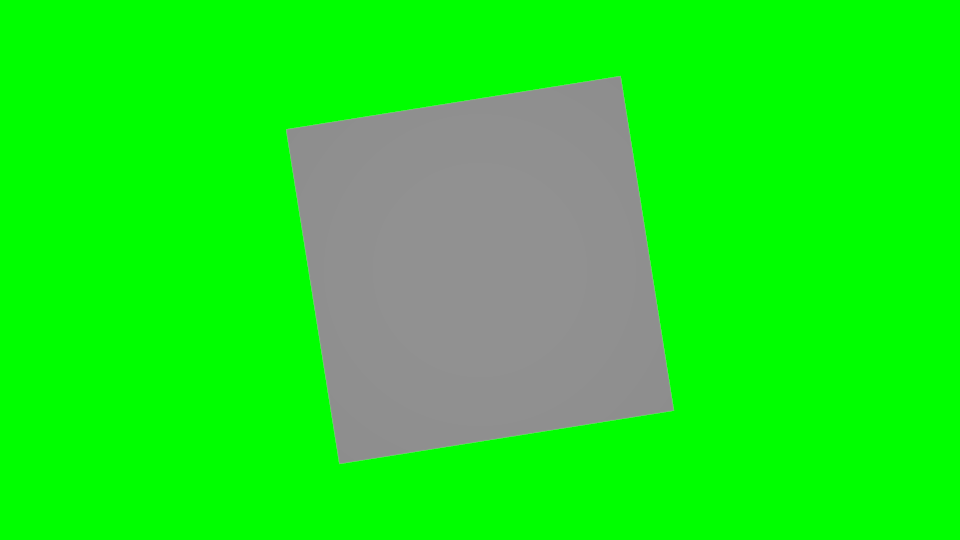
\includegraphics[width=.25\textwidth]{../images/cube_03/0010.png}
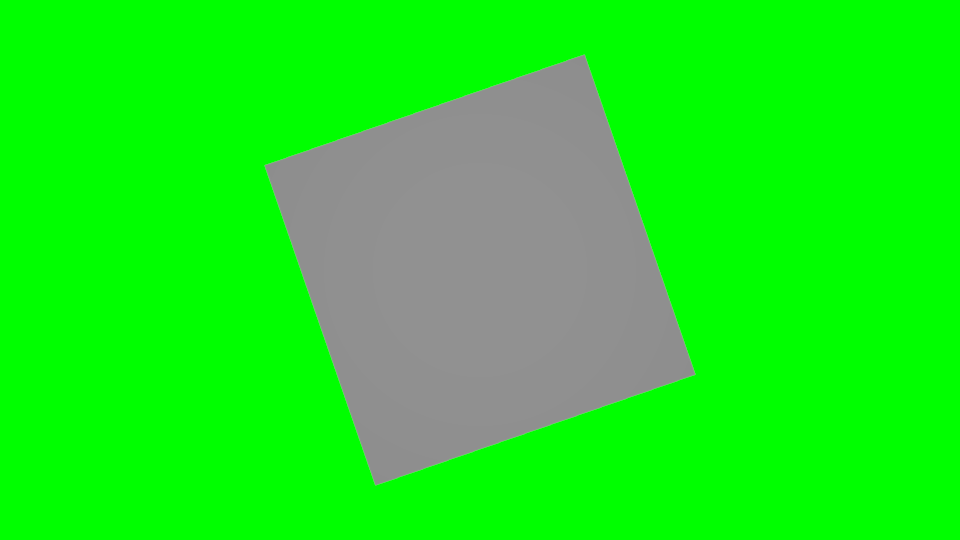
\includegraphics[width=.25\textwidth]{../images/cube_03/0020.png}
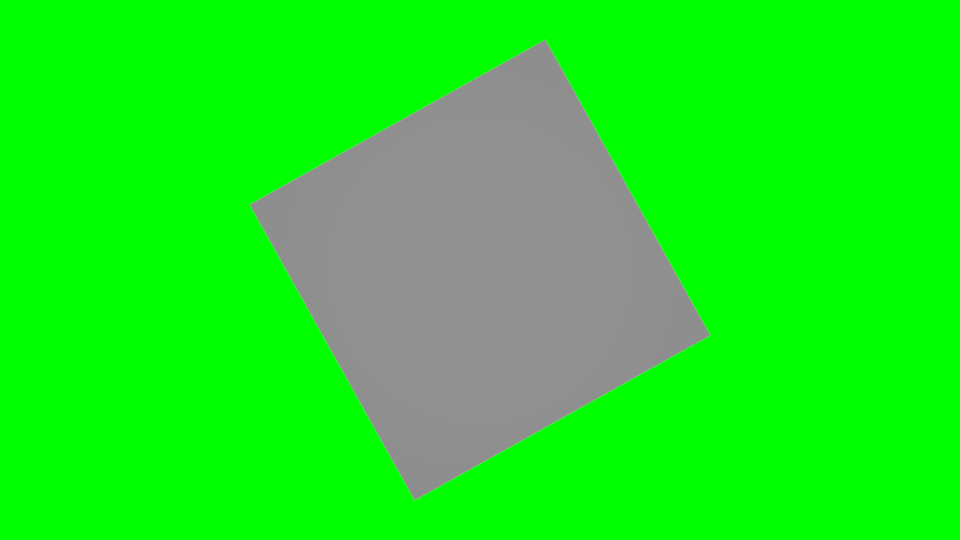
\includegraphics[width=.25\textwidth]{../images/cube_03/0030.png}

\includegraphics[width=.25\textwidth]{../images/cube_03/0040.png}
\caption[]{2D image derived from 3D cube}
\label{fig:2dCube3}
\end{figure}

\subsection{Contour detection}
There are different ways to extract the features of an object. As for this project we used a contour detection to extract the main features from the object. This way we received enough information from the object to compare with, but we didn't overcomplicated the problem. As is described in~\autocite{Lanser95robustvideo-based} , there a more complicated but robust ways to better extract features from an object. Though with the current time limit, we didn't pursue this method. As can be seen further in this report, the current method used was, how crude it might be, sufficient for the problem at hand.
For the contour method we used OpenCV. This library provided us with tested methods to use and enough flexibility to be tailored for our problem.
First the received image is converted to a gray scaled image. As can be seen in~\autocite{5329404} , using a RGB image over Gray scaled image will not increase the accuracy by much. \enquote{Almost 90\% of edge information in a colour image can be found it the corresponding gray scaled image.} So in compliance with the K.I.S.S.~\footnote{Stands for "Keep it simple, stupid" or "Keep it short and simple"} principle, we used a gray scaled image which is also a prerequisite to be able to use the standard contour detection build in OpenCV. Figure~\ref{fig:SphereContour} shows the end result of the contour detection on a 2D converted image from the sphere.

\begin{figure}[h!]
\center
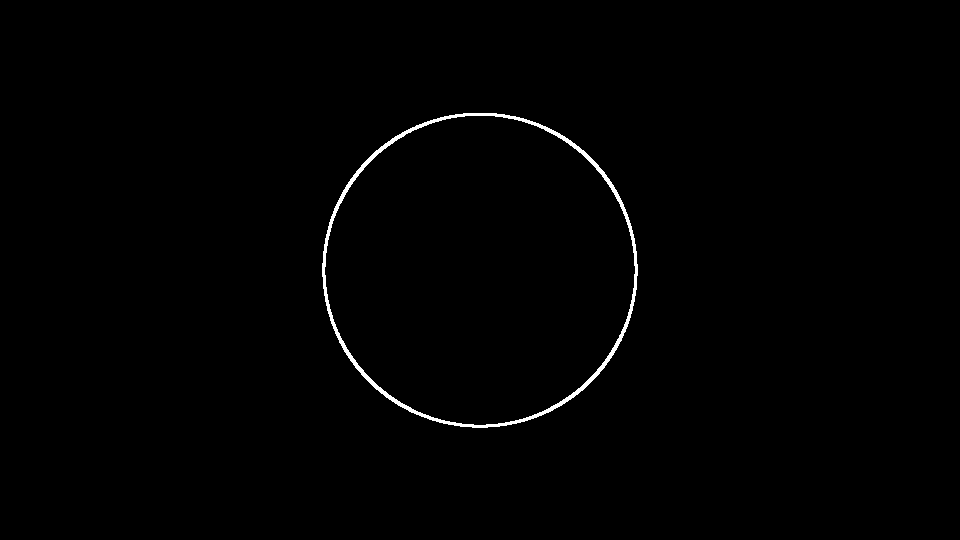
\includegraphics[width=.5\textwidth]{../images/contour_sphere.png}
\caption[]{Contour detection from sphere}
\label{fig:SphereContour}
\end{figure}

\section{Camera}
For this project we use a BubleBee2 and an Asus XTion Pro (also known as a "Kinect"). Each of these cameras have their own features which are usable in different parts of the project. Figure~\ref{fig:camera} shows the result of using the Kinect camera. The cameras shows us the workplace of the robot. The vision part here is to detect the object derived from the video feed. Detecting the object can be done in several ways. For this project we already have a image of the contours of the object we're searching for. This gives us one way of searching for it.

\begin{figure}[h!]
\center
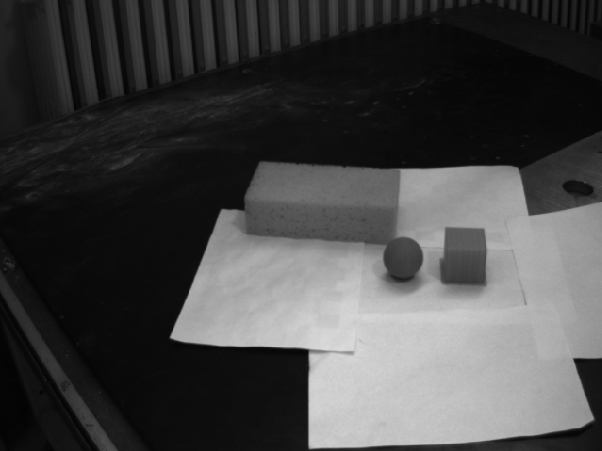
\includegraphics[width=.4\textwidth]{../images/camera_left.png}
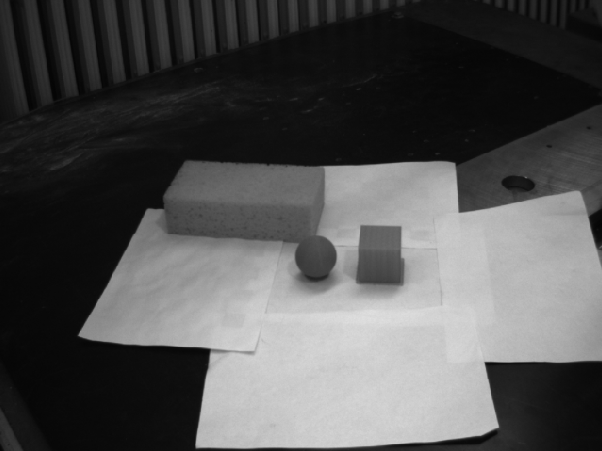
\includegraphics[width=.4\textwidth]{../images/camera_right.png}
\caption[]{Kinect Camera}
\label{fig:camera}
\end{figure}

\subsection{Colour segmentation}
As the colour of the object is already known, to perform a colour segmentation on the video feed is a logical step to take. This will exclude any other objects that has nothing to do with the object we're searching for. If the object was build using multiple colours, using a colour segmentation method would still be valuable as long as there are not too much interference of overlapping colours. This object doesn't have any colour patterns, which you could have also used otherwise, but it consist of one colour. This makes this step a bit easier, though detecting an object with multiple colour would have been a nice expansion.
For this object, the cube has the same colour, we returned a thresholded image which only contains the colours in a range between H=0-179, S=130-255 and V=80-255. As shadows and different light conditions have an effect on the result, detecting the colour within a certain range is necessary. This result will then be (morphological) opened and closed in order to remove any small irregularities.
Figure~\ref{fig:colourSphere} shows the end result.

\begin{figure}[h!]
\center
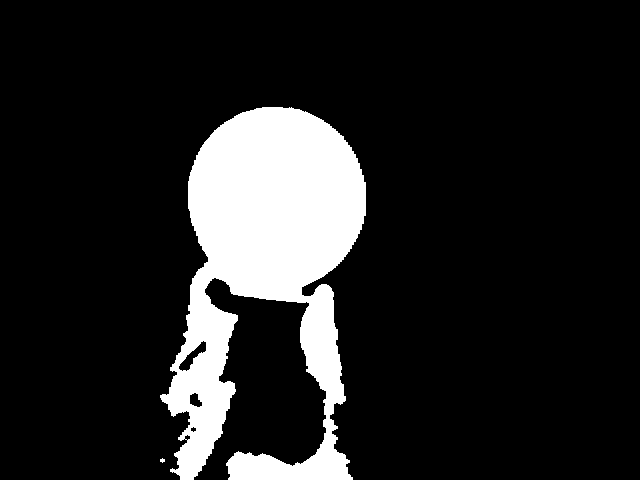
\includegraphics[width=.5\textwidth]{../images/colour_sphere.png}
\caption[]{Colour detection}
\label{fig:colourSphere}
\end{figure}

\subsection{Contour detection}
The contour detection used on the video feed is the same one used for the 2D image of the object. Only minor changes where necessary in order to change the video feed to the correct colour space. See Figure~\ref{fig:colourContourSphere} for the result of the contour detection after a colour segmentation.

\begin{figure}[h!]
\center
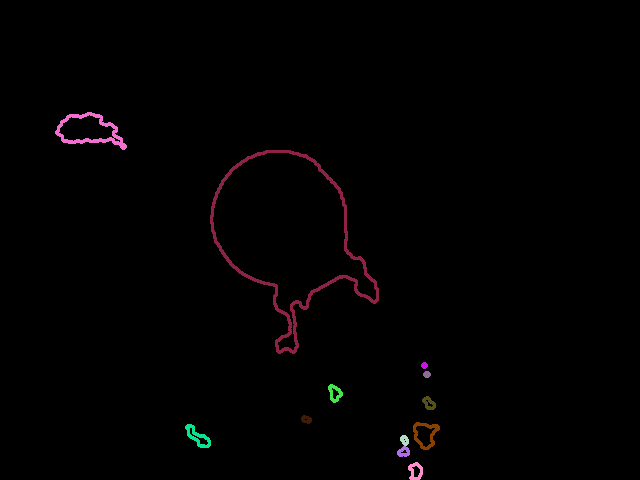
\includegraphics[width=.5\textwidth]{../images/colourContour_sphere.png}
\caption[]{Colour contour detection}
\label{fig:colourContourSphere}
\end{figure}

\section{Feature detection}
The feature detection uses several different methods in order to compare features from the 2D image to the converted video feed. The feature detection mainly consist of a SURF algorithm with a FLANN matcher.

\subsection{SURF}
To detect features from an image, a SURF algorithm is performed on both the object as the scene (i.e. video feed). SURF stands for Speeded Up Robust Features detection method. SURF was inspired from the SIFT algorithm but is several times faster. As for this part we're using a live feed, the speed of the algorithm is crucial. OpenCV has a SURF implementation which we used for this project. We used SURF with an hessian threshold of 400. This resulted in enough keypoints to use for the comparison.

\subsection{FLANN matcher}
FLANN stands for Fast Approximate Nearest Neighbor Search Library. FLANN is a library for performing fast approximate nearest neighbor searches. The algorithm used to match points from the object and scene is based on this. The used FlannBasedMatcher function trains the descriptor collection and find the best matches~\autocite{FlannBasedMatcher} . After finding the best matches, a quick calculation is done between the keypoint distances. In the end only matches who aren't too far away from each other are considered "good" matches and are used. The end result is then drawn and can be seen in Figure~\ref{fig:colourContourFeatureSphere}.

\begin{figure}[h!]
\center
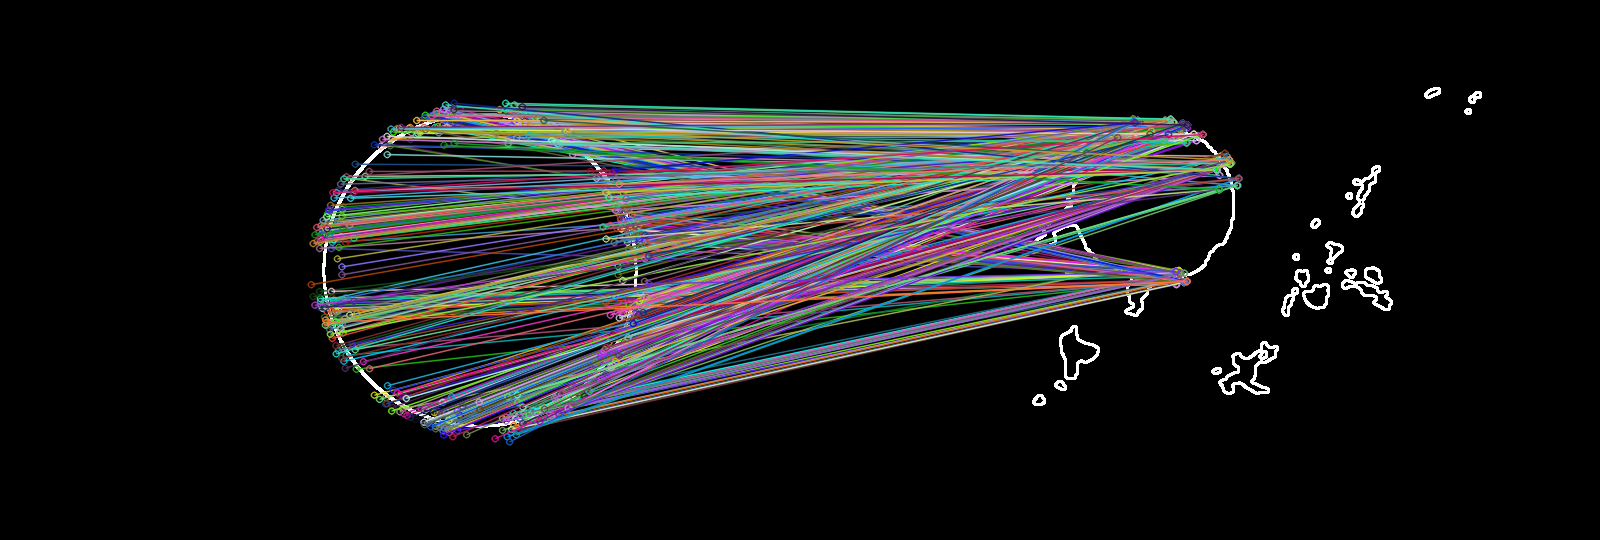
\includegraphics[width=1.0\textwidth]{../images/colourContourFeature_sphere.png}
\caption[]{Colour contour detection}
\label{fig:colourContourFeatureSphere}
\end{figure}

\section{ROS}
The connection with ROS comes down to receiving the video feed from different cameras and publishing information. After this Vision part, combined with the information received from calibrating the robot and camera, we can give the Robotics side coordinate of the wanted object. The Robotics part then can calculate how it needs to move in order to pick the object and place it somewhere else. This is further discussed in the Chapter Calibration and the Chapter Robotics.

\subsection{PCL}
text

\chapter{Wrapping Up}
\section{Conclusion}
%\section{Conclusion}
text

\printbibliography
\addcontentsline{toc}{chapter}{Bibliography}
\end{document}